\documentclass[a4paper]{article}
\usepackage[english, russian]{babel} % русский язык
\usepackage[utf8]{inputenc} % русский язык
\usepackage{graphicx} % вставка изображений
\graphicspath{{images/}} % папка с изображениями

\usepackage{multicol} % несколько колонок
\usepackage[rightcaption]{sidecap}
\usepackage[top=1.5cm]{geometry}
\usepackage{tabularx} % растянуть таблицу
\usepackage{array} % растянуть таблицу
\usepackage{fancyhdr}
\usepackage{caption}

\pagestyle{fancy}
\fancyhead{}
\fancyfoot{}
\fancyfoot[R]{\thepage}

\setlength{\textfloatsep}{1pt}

\begin{document}
\setcounter{page}{23}
\begin{figure}[h]
    \centering
    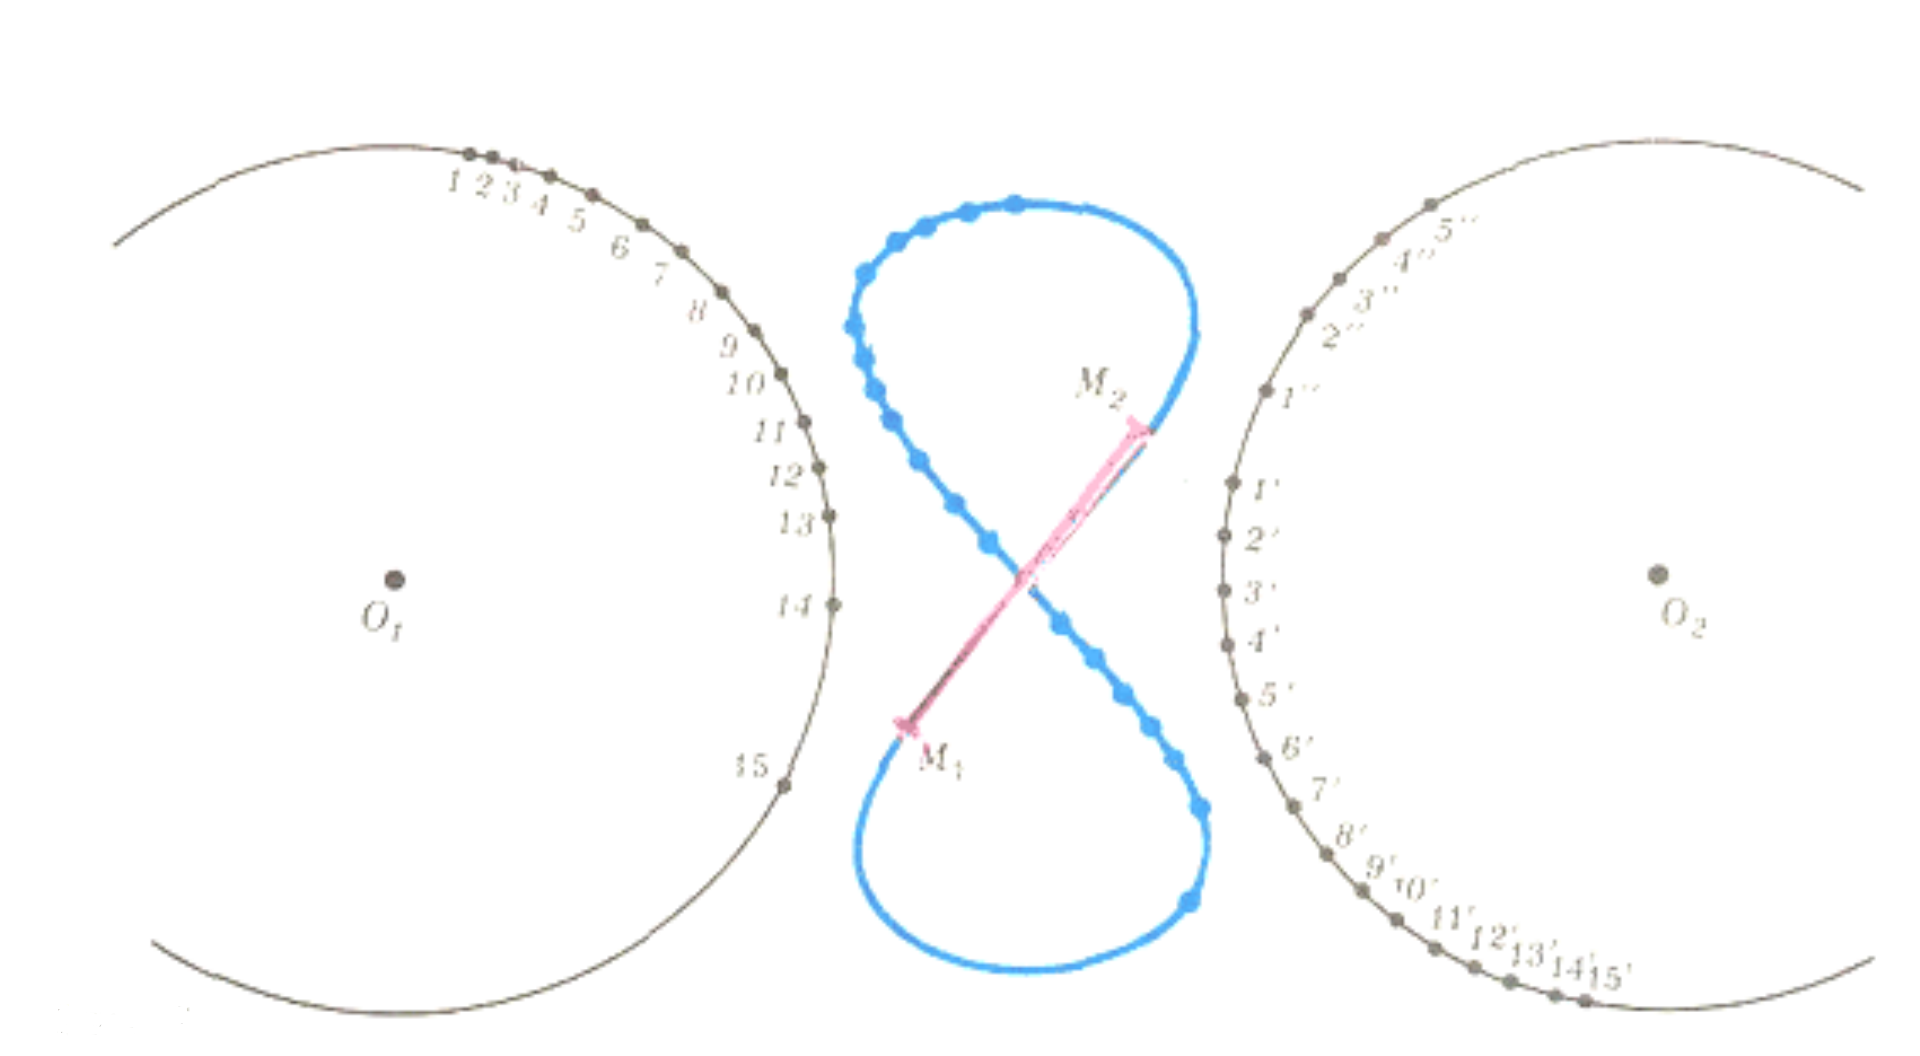
\includegraphics[width=0.92\textwidth]{scheme.png}
    \caption*{\raggedright \textbf{Рис. 7}}
    \label{fig:example}
\end{figure}

\begin{multicols}{2}
    	% Вводите текст в первую колонку
    	\fontsize{11}{12}\selectfont{{Точки A1 и A2 могут перемещаться по окружностям радисуса R с центрами O1 и O2. Заметим, что наибольшее возможное значение расстояния |A1A2| равно 2(l + R)(рис. 5,a), а наименьшее - 2(l - R) (при l >= R) или 0 (при l <= R) (рис. 5, а, б). Отсюда следует, что для существования механизма Уатта необходимо, чтобы параметры d, R и l удовлетворяли неравенствам 

l - r <= d <= l + R.

	Мы будем говорить, что участок M1M2 кривой отличается от отрезка прямой |M1M2| не более, чем на k \%, если каждая точка M этого участка кривой удалена от отрезка M1M2 на расстояние, не превосходящее a0 = k/100|M1M2|(имеется в виду длина перпендикуляра из точки M на отрезок M1M2; рис. 6).

	Теперь всё готово для того, чтобы сформулировать задание математического практикума.\smallskip

\noindent{\textbf{Задание}}

\noindent{По параметрам d, R и l (см. таблицу) плоского шарнирного механизма Уатта:}

	a) начертите по точкам кривую Уатта, описываемую серединой шатуна;

	б) на построенной траектории при помощи линейки определите длину наибольшего участка кривой, отличающегося от отрезка прямой менее чем на 5 \%.

\noindent{\textbf{Образец}}

	d = 3; R = 4; l = 5 (рис. 5).}}

	
	\fontsize{8}{10}\selectfont{З а м е ч а н и е. Для самостоятельной работы возьмите один (или несколько) из наборов значений d, R, l из таблицы. Положение точки М нужно находить при помощи циркуля и линейки: поставив одну ножку циркуля с раствором 2d в некоторую точку Р окружности с центром в точке O1, радиуса R, искать другой ножкой точку Q на второй окружности (с центром O2 радиуса R); середина отрезка [PQ] определяется при помощи линейки. Число точек Р, которое нужно взять для более или менее точного построения искомой траектории, равно 15; при вычерчивании кривой по построенным точкам нуж нужно помнить о ее симметрии.

	После того как вы построите кривую, попробуйте ответить на несколько вопросов. 
	
1 deg На готовом чертеже покажите «полный цикл работы» механизма (т. е. то, как пе мещается шатун, когда его середина движет ся по кривой Уатта).

2 deg Сколько у данного механизма существует положений, из которых можно на чать движение более чем двумя способами?}
\end{multicols}
\footnotesize{{\begin{table}[h!]
	\caption*{\raggedright Т а б л и ц а}
	\centering
    	\begin{tabularx}{\textwidth}{|>{\centering \arraybackslash}X|*{13}{>{\centering \arraybackslash}X|}}
        		\hline \rule{0cm}{0.8 cm} \centering
        		d&4&4&1&1&2&1&1&4&13&3&2&4 \\ \hline \rule{0cm}{0.8 cm} \centering
        		R&3&8&6&5&3&2&3&3&12&4&3&7 \\ \hline \rule{0cm}{0.8 cm} \centering
        		l&5&5&5&2&2&1&1&2&5&2&1&2 \\ \hline
    	\end{tabularx}
\end{table}}
\end{document}
